\documentclass[10pt]{article}

\RequirePackage{amsmath}
\RequirePackage{amsthm}
\RequirePackage{amssymb}
% \RequirePackage[top=2cm, asymmetric, left=2.5cm, right=6cm]{geometry}
\RequirePackage[top=2cm]{geometry}

\RequirePackage{titlesec}
\RequirePackage[hidelinks]{hyperref}
\RequirePackage[english]{babel}
\RequirePackage[autostyle, english=american]{csquotes}
\RequirePackage[skip=8pt]{parskip}
\RequirePackage{caption}
\RequirePackage[nodisplayskipstretch]{setspace}
\RequirePackage[dvipsnames, table]{xcolor}
\RequirePackage{tikz}
\RequirePackage{tcolorbox}
\RequirePackage{enumitem}
\RequirePackage{multicol}

\RequirePackage{graphicx}
\graphicspath{{./media/}}

% \RequirePackage{mleftright}
% \mleftright

% \RequirePackage{cmbright}

\RequirePackage{libertine}
\RequirePackage{libertinust1math}

\usepackage{inconsolata}

\input{style.tex}
\newcommand{\probability}[1]{\ensuremath{\operatorname{P} \left( #1 \right)}}
\newcommand{\expected}[1]{\ensuremath{\operatorname{E} \left( #1 \right)}}
\newcommand{\variance}[1]{\ensuremath{\operatorname{Var} \left( #1 \right)}}
\newcommand{\given}[1][]{\ensuremath{\: #1\vert \:}}


\title{AP Statistics Notes}
\author{Rushil Surti}

\begin{document}

\maketitle
\newpage

\section{Exploring One-Variable Data}

Much of the start of this chapter is quite redundant and self-explanatory in
terms of how to read, organize, and apply graphs and tables of data, so I
really won't be taking notes on that stuff.

\begin{blackbox}
    \begin{definition}
        A \textbf{marginal distribution} is a distribution which looks at the "margins" of the table, and gives the absolute or relative frequency of totals of rows or columns.
    \end{definition}
\end{blackbox}

\begin{example}
    Consider the following table, detailing the number of individuals of type \( A \) or \( B \) with properties \( C \) or \( D \).

    \begin{center}
        \begin{tabular}{c|c|c|c}
            & \( C \) & \( D \) & (Total) \\
            \hline \( A \) & 3 & 1 & \cellcolor{yellow!30} 4 (44.4\%) \\
            \hline \( B \) & 4 & 1 & \cellcolor{yellow!30} 5 (55.6\%) \\
            \hline (Total) & \cellcolor{blue!20} 7 (77.8\%) & \cellcolor{blue!20} 2 (22.2\%) & 9
        \end{tabular}
    \end{center}

    Both the blue and yellow squares represent marginal distributions, with (for instance) the first blue square representing the marginal distribution of individuals with property \( C \).
\end{example}

\begin{blackbox}
    \begin{definition}
        A \textbf{conditional distribution} is a distribution which looks at the distribution of the population given some condition (or property) \( P \).
    \end{definition}
\end{blackbox}

\begin{example}
    Using the same table, we will look at the conditional distribution of individuals given they have property \( C \).

    \begin{center}
        \begin{tabular}{c|c|c|c}
            & \( C \) & \( D \) & (Total) \\
            \hline \( A \) & \cellcolor{ForestGreen!20} 3 (42.9\%) & 1 & 4 \\
            \hline \( B \) & \cellcolor{ForestGreen!20} 4 (57.1\%) & 1 & 5 \\
            \hline (Total) & 7 & 2 & 9
        \end{tabular}
    \end{center}
\end{example}

We can also describe the shape of distributions, classifying into a few major categories. For now, we will only be describing them by their general shape, but later we will apply mathematical methods (I think) to see which one best describes each. Below are the five major shapes of distributions:

\begin{itemize}
    \item \textbf{Symmetric Distribution}: One that has a peak in the center and is roughly symmetric about this center. Note that while other distributions may be symmetric about some center (see the Bimodal Distribution), we are in particular looking for this bell curve sort of shape.

    \begin{center}
    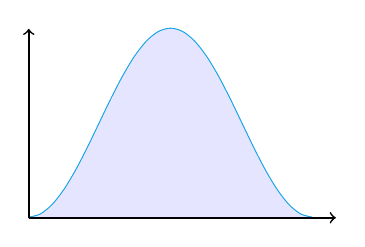
\begin{tikzpicture}[domain=0:6, scale=0.6]
        \draw[color=Cerulean, thick, smooth] plot (\x, {-2 * cos((\x / 6 * 2 * pi) r) + 2});
        \fill[color=blue!10, smooth] (0, 0) -- plot (\x, {-2 * cos((\x / 6 * 2 * pi) r) + 2}) -- (6, 0) -- cycle;

        \draw[semithick, ->] (0, 0) -- (6.5, 0);
        \draw[semithick, ->] (0, 0) -- (0, 4);
    \end{tikzpicture}
    \end{center}

    \item \textbf{Left Skewed Distribution}: One which has a peak on the right side and trails off down to the left.

    \begin{center}
    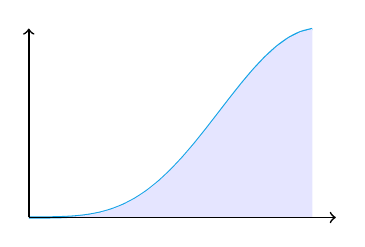
\begin{tikzpicture}[domain=0:6, scale=0.6]
        \draw[color=Cerulean, thick, smooth] plot (\x, {(sin((\x - 3) / 2 r) + 1)^2});
        \fill[color=blue!10] (0, 0) -- plot (\x, {(sin((\x - 3) / 2 r) + 1)^2}) -- (6, 0) -- cycle;

        \draw[semithick, ->] (0, 0) -- (6.5, 0);
        \draw[semithick, ->] (0, 0) -- (0, 4);
    \end{tikzpicture}
    \end{center}

    \item \textbf{Right Skewed Distribution}: One which has a peak on the left side and trails off down to the right.

    \begin{center}
    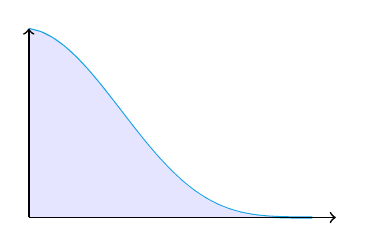
\begin{tikzpicture}[domain=0:6, scale=0.6]
        \draw[color=Cerulean, thick, smooth] plot (\x, {(-sin((\x - 3) / 2 r) + 1)^2});
        \fill[color=blue!10] (0, 0) -- plot (\x, {(-sin((\x - 3) / 2 r) + 1)^2}) -- (6, 0) -- cycle;

        \draw[semithick, ->] (0, 0) -- (6.5, 0);
        \draw[semithick, ->] (0, 0) -- (0, 4);
    \end{tikzpicture}
    \end{center}

    \item \textbf{Bimodal Distribution}: One which has peaks on both the right and left side, dropping down at the center.

    \begin{center}
    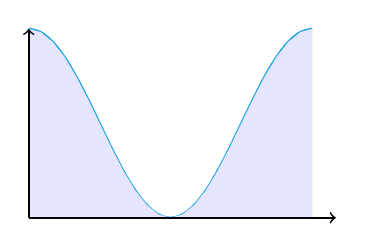
\begin{tikzpicture}[domain=0:6, scale=0.6]
        \draw[color=Cerulean, thick, smooth] plot (\x, {4 * cos((pi * \x / 6) r)^2});
        \fill[color=blue!10] (0, 0) -- plot (\x, {4 * cos((pi * \x / 6) r)^2}) -- (6, 0) -- cycle;

        \draw[semithick, ->] (0, 0) -- (6.5, 0);
        \draw[semithick, ->] (0, 0) -- (0, 4);
    \end{tikzpicture}
    \end{center}

    \item \textbf{Uniform Distribution}: One which is roughly consistent for all values.

    \begin{center}
    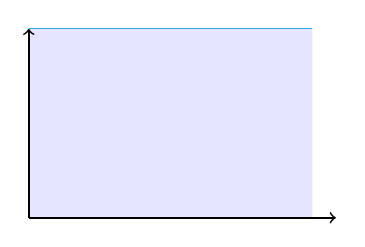
\begin{tikzpicture}[domain=0:6, scale=0.6]
        \draw[color=Cerulean, thick, smooth] plot (\x, {4});
        \fill[color=blue!10] (0, 0) -- plot (\x, {4}) -- (6, 0) -- cycle;

        \draw[semithick, ->] (0, 0) -- (6.5, 0);
        \draw[semithick, ->] (0, 0) -- (0, 4);
    \end{tikzpicture}
    \end{center}
\end{itemize}

There is also some more general terms that we can use to further describe parts of distributions.

\begin{blackbox}
    \begin{definition}
        A \textbf{cluster} is an area on the distribution where this a high
        amount or the majority of the data near this point. A \textbf{gap} is
        an area on the distribution where there is no data. This also goes in
        hand with \textbf{outliers}, which are data points offset from the
        general distribution, usually separated by gaps and found at the
        extremities. A \textbf{peak} as we have seen before is a high point on
        the distribution. The spread (or variability) of the graph can be
        described by the \textbf{range}, or the difference between the highest
        and lowest values in the data.
    \end{definition}
\end{blackbox}

Generally on the AP test and such when you're asked to \textit{describe} a
distribution, there are four major things you must find.

\begin{enumerate}
    \item \textbf{Shape}: These are described above (symmetric, left/right skewed, etc.).
    \item \textbf{Center}: This can be described with the mean or the median.
    \item \textbf{Spread}: These are described through the range, interquartile range, mean absolute deviation, standard deviation, etc. (These will come up later?)
    \item \textbf{Outliers}: Talk about whether there are or aren't any potential outliers in the data.
\end{enumerate}

When you're asked to \textit{compare} two or more distributions of data, look
at and compare the centers and spread.

Note that in some cases it is not always applicable to simply draw conclusions
based on the numerical values of the range and such, so be on the lookout and
intuit the information yourself.

\begin{blackbox}
    \begin{definition}
        The \textbf{IQR}, or \textbf{interquartile range}, of a given data set
        is found by taking the medians \( M_1 \) of upper half and \( M_2 \)
        lower half of the set and finding their difference \( M_1 - M_2 \).
        This is another measure of spread.
    \end{definition}
\end{blackbox}

\begin{example}
    The IQR of the data set \( 1, 1, 2, 5, 7, 8, 9 \) is \( 7 \). Because the
    median of \( 7, 8, 9 \) minus the median of \( 1, 1, 2 \) is \( 7 \).

    The IQR of the data set \( 2, 4, 6, 8 \) is \( 4 \) because the median of \( 6, 8 \) minus the median of \( 2, 4 \) is \( 4 \).
\end{example}

Often in statistics, we cannot take into account or measure data for an entire
population. In this case, we rely on taking \textbf{samples}, or smaller
groups, from this greater population and making generalizations to the entire
population based on the statistics from these smaller groups. When consider
samples however, we sometimes do have to make adjustments to how we interpret
summary statistics, in particular variance and standard deviation.

\begin{blackbox}
    \begin{definition}
        The \textbf{standard deviation} of an entire popluation with \( n \) data points, denoted by \( \sigma \), is given by the following:
        \[
            \sigma = \sqrt{\frac{\sum_{i = 1}^n \left( X_i - \mu  \right)^2}{n}},
        \]
        where \( X_i \) and \( \mu \) denote the \( i \)th value in population
        and the mean of the entire population, respectively.

        The \textbf{sample standard deviation}, however is slightly different. Let the mean of the sample be \( \overline{X} \) and the size be \( n \). Then the sample standard deviation, denoted with \( S \) is
        \[
            S = \sqrt{\frac{\sum_{i = 1}^n \left( X_i - \overline{X} \right)^2}{n - 1}}.
        \]

        To calculate variance, simply square the standard deviation.
    \end{definition}
\end{blackbox}

Notice the \( n - 1 \) in the denominator for the samples. This is used to
correct for bias in measurement.\footnote{Right now, the exact specifics as to
how and why are kind of fuzzy for me but here's a resource?
\url{https://stats.stackexchange.com/questions/3931/intuitive-explanation-for-dividing-by-n-1-when-calculating-standard-deviation}}

Generally when there exists outliers in the data, the median and interquartile
range are better choices for center and spread, while mean and standard
deviation are better for when there is more symmetric data without outliers.

Note we have that for any linear transformation \( T \colon X_i \mapsto a X_i +
b \) and set of data \( M \) the following (trivial to prove):
\begin{align*}
    \mu \left( T \left( M \right) \right) &= T \left( \mu \left( M \right) \right) \\
    \sigma \left( T \left( M \right) \right) &= a \left( \sigma \left( M \right) \right) \\
    \operatorname{Med} \left( T \left( M \right) \right) &= T \left( \operatorname{Med} \left( M \right) \right) \\
    \operatorname{IQR} \left( T \left( M \right) \right) &= a \operatorname{IQR} \left( M \right)
\end{align*}
In general, measures of centers should transform exactly under a linear
transformation, while measures of spread and range should only transform under
stretches (not translations).

\begin{blackbox}
    \begin{definition}
        When calculating these center and spread values for a \colorbox{Cerulean}{p}opulation we
        call them \textbf{\colorbox{Cerulean}{p}arameters}

        When we calculate them for a \colorbox{ForestGreen}{s}ample of the
        population, they are called \textbf{\colorbox{ForestGreen}{s}tatistics}.
    \end{definition}
\end{blackbox}

By convention, we consider any data point \( X \) an outlier when \( X < Q_1 -
1.5 \cdot IQR \) or \( X > Q_3 + \cdot 1.5 \cdot IQR \), where \( Q_1 \) and \(
Q_3 \) denote the first and third quartile respectively.

\begin{blackbox}
    \begin{definition}
        A \textbf{percentile} is defined as either the percentage of data below
        a certain value in the data, or the percentage of data below
        \textit{and including} a certain value in the data.
    \end{definition}
\end{blackbox}

\begin{example}
    The percentile rank of the value of \( 3 \) in the following data set is
    either \( 50\% \) or \( 75\% \) depending on definition\footnote{While the
        difference may seem large here, statisticians are fine with this
        somewhat lack of consensus on percentiles because the difference is
        quite negligible for large samples/populations}:
    \[
        1, 1, 3, 4
    .\]
\end{example}

This goes in tandem with cumulative relative frequency graphs.

\begin{blackbox}
    \begin{definition}
        A \textbf{cumulative relative frequency graph} is a graph that, given a
        corresponding \( x \)-value, tells one the percentage of values below
        that \( x \)-value in the set of data. This function, which we will denote \( f \left( x \right) \), is a strictly increasing bijection from the range of the data to the interval \( \left[ 0, 1 \right] \) such that \( f \left( a \right) = 0 \) and \( f \left( b \right) = 1 \).
    \end{definition}
\end{blackbox}

One very common tool in statistics is the notion of a \( z \)-score.

\begin{blackbox}
    \begin{definition}
        The \( z \)-score of a certain data point \( x \) is the number of
        standard deviations it is away from the mean. Numerically, that is:
        \[
            z = \frac{x - \mu}{\sigma}
        .\]
    \end{definition}
\end{blackbox}

This measure is used to tell us how often something occurs and can be useful to
help make inferences.

Oh boy it's time for some continuity now.

\begin{blackbox}
    \begin{definition}
        A \textbf{density function} or \textbf{density curve} is a continuous function \( f \left( x \right) \) defined on an interval \( \left[ a, b \right] \) such that
        \[
            \int_{a}^{b} f \left( x \right) \, dx = 1
        .\]
    \end{definition}
\end{blackbox}

\begin{center}
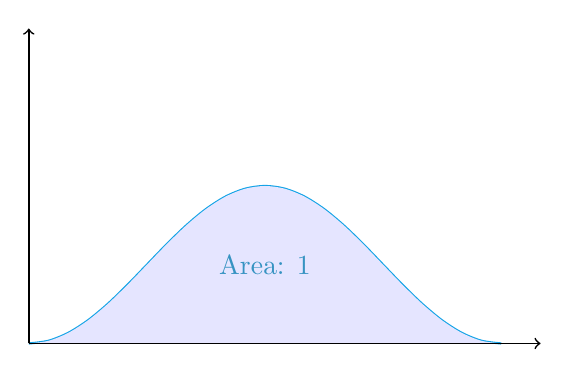
\begin{tikzpicture}[domain=0:6, scale=1]
    \draw[color=Cerulean, thick, smooth] plot (\x, {-1 * cos((\x / 6 * 2 * pi) r) + 1});
    \fill[color=blue!10, smooth] (0, 0) -- plot (\x, {-1 * cos((\x / 6 * 2 * pi) r) + 1}) -- (6, 0) -- cycle;

    \draw[semithick, ->] (0, 0) -- (6.5, 0);
    \draw[semithick, ->] (0, 0) -- (0, 4);

    \node[color=Cerulean!80!black] at (3, 1) {Area: \( 1 \)};
\end{tikzpicture}
\end{center}

This is the continuous equivalent of a relative frequency graph and allows us
to model data on a continuous spectrum of values and use our very nice tools of
analysis and such to describe what is going on. For instance, the area under
the curve in a specific interval (something given to us by the integral) gives
the density or probability of data being in the interval.

We can also determine median, mean, and skew graphically from these density
curves. The median line is one which splits the area of the curve exactly into
equal halves on each side, while the mean is the average value, or weighted
sum, of this curve. The location of where the mean and median line are relative
to each other determine the skew on the graph. When the mean is to the right of
the median, we call this right-skewed, and the other way around is called
left-skewed (terms we are already familiar with). For symmetric distributions,
the median and mean are roughly the same, meaning that they aren't skewed.

\begin{multicols}{3}
\begin{center}
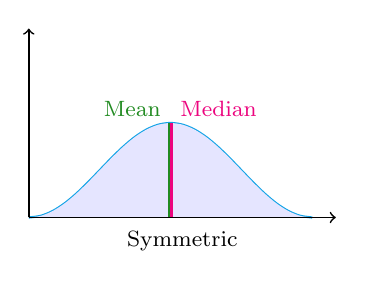
\begin{tikzpicture}[domain=0:6, scale=0.6]
    \draw[color=Cerulean, thick, smooth] plot (\x, {-1 * cos((\x / 6 * 2 * pi) r) + 1});
    \fill[color=blue!10, smooth] (0, 0) -- plot (\x, {-1 * cos((\x / 6 * 2 * pi) r) + 1}) -- (6, 0) -- cycle;

    \draw[very thick, color=ForestGreen] (2.975, 0) -- (2.975, 2);
    \draw[very thick, color=RubineRed] (3.025, 0) -- (3.025, 2);
    \node[anchor=east, color=ForestGreen] at (3, 2.3) {\footnotesize Mean};
    \node[anchor=west, color=RubineRed] at (3, 2.3) {\footnotesize Median};

    \draw[semithick, ->] (0, 0) -- (6.5, 0);
    \draw[semithick, ->] (0, 0) -- (0, 4);

    \node at (3.25, -0.5) {\footnotesize Symmetric};
\end{tikzpicture}
\end{center}

\begin{center}
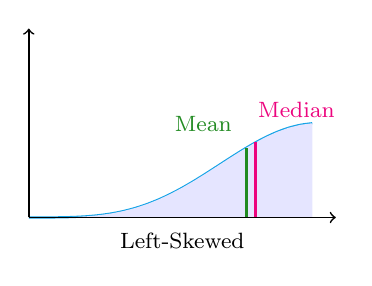
\begin{tikzpicture}[domain=0:6, scale=0.6]
    \draw[color=Cerulean, thick, smooth] plot (\x, {0.5 * (sin((\x - 3) / 2 r) + 1)^2});
    \fill[color=blue!10] (0, 0) -- plot (\x, {0.5 * (sin((\x - 3) / 2 r) + 1)^2}) -- (6, 0) -- cycle;

    \draw[very thick, color=ForestGreen] (4.60993567569, 0) -- (4.60993567569, 2.961 / 2);
    \draw[very thick, color=RubineRed] (4.797, 0) -- (4.797, 3.177 / 2);
    \node[anchor=east, color=ForestGreen] at (4.5, 2.961 / 2 + 0.5) {\footnotesize Mean};
    \node[anchor=west, color=RubineRed] at (4.65, 3.177 / 2 + 0.7) {\footnotesize Median};

    \draw[semithick, ->] (0, 0) -- (6.5, 0);
    \draw[semithick, ->] (0, 0) -- (0, 4);

    \node at (3.25, -0.5) {\footnotesize Left-Skewed};
\end{tikzpicture}
\end{center}

\begin{center}
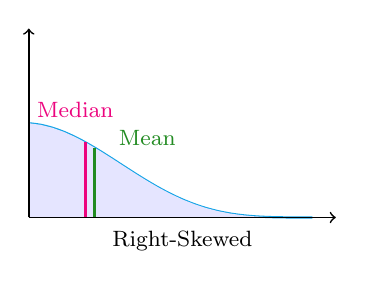
\begin{tikzpicture}[domain=0:6, scale=0.6]
    \draw[color=Cerulean, thick, smooth] plot (\x, {0.5 * (-sin((\x - 3) / 2 r) + 1)^2});
    \fill[color=blue!10] (0, 0) -- plot (\x, {0.5 * (-sin((\x - 3) / 2 r) + 1)^2}) -- (6, 0) -- cycle;

    \draw[very thick, color=ForestGreen] (6 - 4.60993567569, 0) -- (6 - 4.60993567569, 2.961 / 2);
    \draw[very thick, color=RubineRed] (6 - 4.797, 0) -- (6 - 4.797, 3.177 / 2);
    \node[anchor=west, color=ForestGreen] at (1.7, 2.961 / 2 + 0.2) {\footnotesize Mean};
    \node[anchor=east, color=RubineRed] at (2, 3.177 / 2 + 0.7) {\footnotesize Median};

    \draw[semithick, ->] (0, 0) -- (6.5, 0);
    \draw[semithick, ->] (0, 0) -- (0, 4);

    \node at (3.25, -0.5) {\footnotesize Right-Skewed};
\end{tikzpicture}
\end{center}
\end{multicols}

The normal distribution, or Gaussian distribution, is one of the most important
and prevalent distributions in statistics. The exact formulations will be
covered later, but the general sense is that it forms a symmetric bell curve shape.

One important idea surrounding the normal distribution is the empirical rule.

\begin{blackbox}
    \begin{definition}
        The \textbf{empirical rule}, or \textbf{\( \mathbf{68} \)-\( \mathbf{95} \)-\( \mathbf{99.7} \) rule} rule tells us that, for a normal distribution there is:
        \begin{itemize}
            \item A \( 68\% \) chance of a value being within one standard deviation of the mean,
            \item A \( 95\% \) chance of a value being within two standard deviations of the mean, and
            \item A \( 99.7\% \) chance of a value being within three standard deviations of the mean.
        \end{itemize}
    \end{definition}
\end{blackbox}

\vspace{0.3cm}

\begin{center}
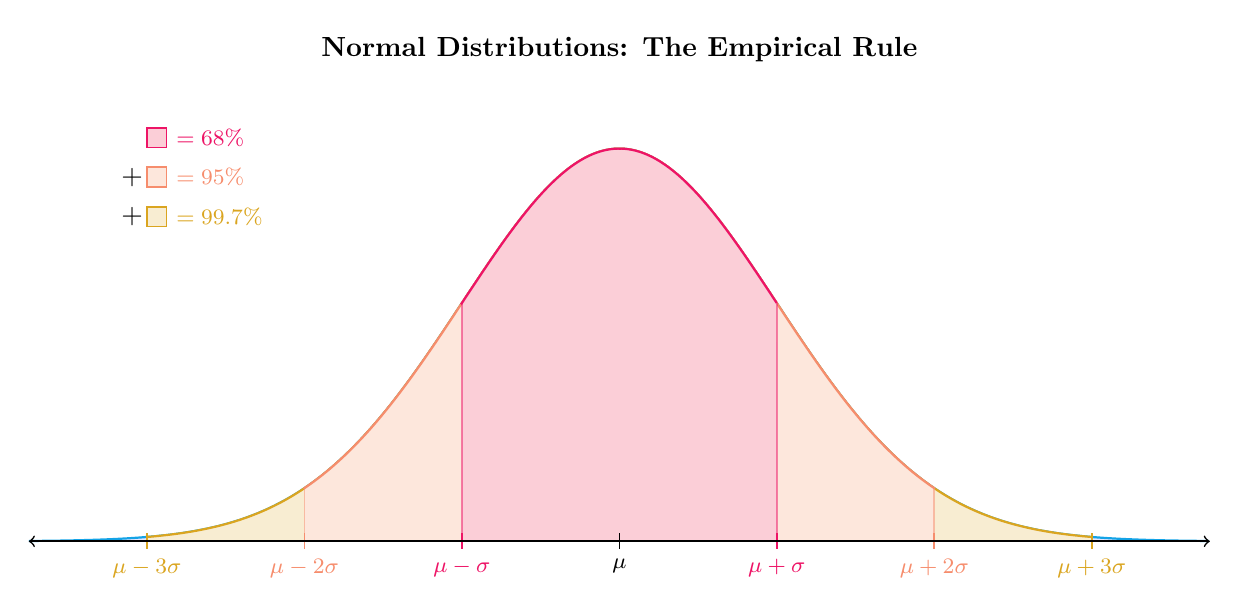
\begin{tikzpicture}[domain=-1.5:1.5, scale=5]
    \fill[color=blue!10, smooth] (-1.5, 0) -- plot (\x, {1/(0.4 * sqrt(2 * pi)) * exp(-1/2 * (\x / 0.4) ^ 2)}) -- (1.5, 0) -- cycle;
    \draw[color=Cerulean, thick, smooth, samples=200] plot (\x, {1/(0.4 * sqrt(2 * pi)) * exp(-1/2 * (\x / 0.4) ^ 2)});

    \fill[color=Goldenrod!20, smooth, domain=-1.2:1.2] (-1.2, 0) -- plot (\x, {1/(0.4 * sqrt(2 * pi)) * exp(-1/2 * (\x / 0.4) ^ 2)}) -- (1.2, 0) -- cycle;
    \draw[color=Goldenrod, thick, smooth, samples=200, domain=-1.202:1.202] plot (\x, {1/(0.4 * sqrt(2 * pi)) * exp(-1/2 * (\x / 0.4) ^ 2)});
    \draw[color=Goldenrod, semithick, draw opacity=0.5] (-1.2, 0) -- (-1.2, 0.0111);
    \draw[color=Goldenrod, semithick, draw opacity=0.5] (1.2, 0) -- (1.2, 0.0111);

    \fill[color=Melon!20, smooth, domain=-0.8:0.8] (-0.8, 0) -- plot (\x, {1/(0.4 * sqrt(2 * pi)) * exp(-1/2 * (\x / 0.4) ^ 2)}) -- (0.8, 0) -- cycle;
    \draw[color=Melon, thick, smooth, samples=200, domain=-0.802:0.802] plot (\x, {1/(0.4 * sqrt(2 * pi)) * exp(-1/2 * (\x / 0.4) ^ 2)});
    \draw[color=Melon, semithick, draw opacity=0.5] (-0.8, 0) -- (-0.8, 0.13498);
    \draw[color=Melon, semithick, draw opacity=0.5] (0.8, 0) -- (0.8, 0.13498);

    \fill[color=WildStrawberry!20, smooth, domain=-0.4:0.4] (-0.4, 0) -- plot (\x, {1/(0.4 * sqrt(2 * pi)) * exp(-1/2 * (\x / 0.4) ^ 2)}) -- (0.4, 0) -- cycle;
    \draw[color=WildStrawberry, thick, smooth, samples=200, domain=-0.402:0.402] plot (\x, {1/(0.4 * sqrt(2 * pi)) * exp(-1/2 * (\x / 0.4) ^ 2)});
    \draw[color=WildStrawberry, semithick, draw opacity=0.5] (-0.4, 0) -- (-0.4, 0.6049);
    \draw[color=WildStrawberry, semithick, draw opacity=0.5] (0.4, 0) -- (0.4, 0.6049);

    \draw[semithick] (0, 0.02) -- (0, -0.02) node[anchor=north] {\footnotesize \( \mu \)};

    \draw[semithick, color=WildStrawberry] (-0.4, 0.02) -- (-0.4, -0.02) node[anchor=north] {\footnotesize \( \mu - \sigma \)};
    \draw[semithick, color=WildStrawberry] (0.4, 0.02) -- (0.4, -0.02) node[anchor=north] {\footnotesize \( \mu + \sigma \)};

    \draw[semithick, color=Melon] (-0.8, 0.02) -- (-0.8, -0.02) node[anchor=north] {\footnotesize \( \mu - 2\sigma \)};
    \draw[semithick, color=Melon] (0.8, 0.02) -- (0.8, -0.02) node[anchor=north] {\footnotesize \( \mu + 2\sigma \)};

    \draw[semithick, color=Goldenrod] (-1.2, 0.02) -- (-1.2, -0.02) node[anchor=north] {\footnotesize \( \mu - 3\sigma \)};
    \draw[semithick, color=Goldenrod] (1.2, 0.02) -- (1.2, -0.02) node[anchor=north] {\footnotesize \( \mu + 3\sigma \)};

    \draw[semithick, <->] (-1.5, 0) -- (1.5, 0);

    \fill[color=WildStrawberry!20] (-1.2, 1.2 - 0.15) rectangle (-1.15, 1.15 - 0.15);
    \draw[semithick, color=WildStrawberry] (-1.2, 1.2 - 0.15) rectangle (-1.15, 1.15 - 0.15);
    \node[anchor=west, color=WildStrawberry] at (-1.2 + 0.05, 1.2 - 0.025 - 0.15) {\footnotesize \( = 68\% \)};

    \node at (-1.2375, 1.075 - 0.15) {\( + \)};
    \fill[color=Melon!20] (-1.2, 1.1 - 0.15) rectangle (-1.15, 1.05 - 0.15);
    \draw[semithick, color=Melon] (-1.2, 1.1 - 0.15) rectangle (-1.15, 1.05 - 0.15);
    \node[anchor=west, color=Melon] at (-1.2 + 0.05, 1.1 - 0.025 - 0.15) {\footnotesize \( = 95\% \)};

    \node at (-1.2375, 0.975 - 0.15) {\( + \)};
    \fill[color=Goldenrod!20] (-1.2, 1.0 - 0.15) rectangle (-1.15, 0.95 - 0.15);
    \draw[semithick, color=Goldenrod] (-1.2, 1.0 - 0.15) rectangle (-1.15, 0.95 - 0.15);
    \node[anchor=west, color=Goldenrod] at (-1.2 + 0.05, 1.0 - 0.025 - 0.15) {\footnotesize \( = 99.7\% \)};

    \node at (0, 1.25) {\textbf{Normal Distributions: The Empirical Rule}};
\end{tikzpicture}
\end{center}
% Hehe this took a while to make but hey it looks nice imo

\section{Exploring Two-Variable Data}

Often we graph two-variable (quantitative) data with scatter plots.

Generally when classifying relationships between two variables, give them three
attributes:
\begin{enumerate}
    \item \textbf{Linearity/Form}: Does the data follow a linear or close to linear relationship? Is it non-linear? Is there no relationship?
    \item \textbf{Strength}: How closely does it follow the shape described?
    \item \textbf{Direction}: Is it going in the positive or negative direction?
    \item \textbf{Outliers}: Are there any potential outliers in the data?
\end{enumerate}

With two-variable data and scatter plots, we can also identify clusters, or
separated groups, of data.

One way to quantify how "linear" a relationship is is to calculate the
correlation coefficient.

\begin{blackbox}
    \begin{definition}
        The \textbf{correlation coefficient}, denoted \( r \), is a value in the interval \( \left[-1, 1 \right] \) calculated as follows:
        \[
            r = \frac{1}{n - 1} \sum_{i = 1}^{n} z_{x_i} z_{y_i}
        ,\]
        where \( n \) denotes the number of samples and \( z_{x_i} \) and \(
        z_{y_i} \) denote the \( z \)-scores of each \( x \) and \( y \) value
        in the sample data set.
    \end{definition}
\end{blackbox}

A correlation coefficient close to \( -1 \) or \( 1 \) tells us that there is a
very strong negative or positive linear relationship respectively; whereas, if
the correlation coefficient is close to \( 0 \), there isn't really a linear
relationship. Sometimes we will square this \( r \) value if all we're
concerned about is the linearity.

Linear regression is concept of trying to best fit a line to a set of data. We
try to minimize the squared-distance from each point to the line. A linear regression line for a data set \( y \) is usually denoted by \( \hat{y} \).

\begin{blackbox}
    \begin{definition}
        The \textbf{residual} is the difference between a data point and the
        point with the same \( x \) lying on the linear regression line.
    \end{definition}
\end{blackbox}

Sometimes we may also separately graph residuals on a residual plot to see how
good of a fit our line is.

In order to actually calculate our regression line, we can do a little but of
math. The slope of the line will be \( r \cdot s_y / s_x \), where \( s \)
denotes the sample standard deviation of the corresponding sets of data.
Intuitively, this slope makes sense, as it represents an average standard
deviation of \( y \) over that of \( x \) and then adjusted by how close the
data fits to a line by \( r \). We also know that the line will pass through
the point \( \left( \overline{x}, \overline{y} \right) \), or the mean point,
so we can now use point-slope formula to solve for the line. 

\begin{blackbox}
    \begin{definition}
        The equation for a \textbf{linear regression line} for a set of bivariate data is
        \[
            \hat{y} = \overline{y} + r \cdot \frac{s_y}{s_x} \left( x - \overline{x} \right)
        .\]
    \end{definition}
\end{blackbox}

\begin{blackbox}
    \begin{definition}
        The value of \( r^2 \), called the \textbf{coefficient of
        determination}, tells us how much of the variation in \( y \) is
        described by the variation in \( x \), and it also gives us a measure
        of how good of a line of fit we have. It is calculated as
        \[
            r^2 = 1 - \frac{SE_{\hat{y}}}{SE_{\overline{y}}}
        ,\]
        where \( SE_{\hat{y}} \) represents the sum of the squared error of all
        points from the regression line (in other words the sum of the squares
        of all residuals), and \( SE_{\overline{y}} \) represents the sum of
        the squared error of all points from the mean.
    \end{definition}
\end{blackbox}

\begin{blackbox}
    The \textbf{standard deviation of residuals} or \textbf{root mean square deviation (RMSD)} is found with the following formula:
    \[
        RMSD = \sqrt{\frac{\sum_{i = 1}^n \left( y_i - \hat{y} \right)^2}{n - 2}}
    .\]
\end{blackbox}

This gives the average residual, or average error between the regression line
prediction and an actual value.

\section{Collecting Data}

When collecting data and planning studies, it is important to identify the
population and the sample groups and interpret how the data acquired from the
sample can be generalized fairly.

Generally when we think of studies, there are a few types that come to mind:
\begin{itemize}
    \item \textbf{Experiment}: These randomly separate people into groups to
        see if there is any statistical relationship between values when giving
        some sort of stimulus to the population.
    \item \textbf{Retrospective Observational Study}: Using past data to analyze and draw conclusions.
    \item \textbf{Sample Survey}: Using current data and surveying to analyze and draw conclusions. This is also an observational study.
    \item \textbf{Propspective Observational Study}: Gathering future data to analyze and draw conclusions.
\end{itemize}

\begin{blackbox}
    \begin{definition}
        An \textbf{explanatory variable} is just an independent variable. A
        \textbf{response variable} is a dependent variable.
    \end{definition}
\end{blackbox}

There are several different types of bias that may slip into the sampling
process that make any conclusions drawn illegitimate:
\begin{itemize}
    \item \textbf{Voluntary Response Sampling}: When you ask people to
        volunteer for something, this may filter out those that don't like
        something, potentially skewing results.

        If a Youtuber asks their viewers to complete a survey on how much they
        like the channel, it's probably going to be biased in favor.

    \item \textbf{Convenience Sampling}: Using samples and data that are the
        easiest to obtain, but not necessarily the most fair.

    \item \textbf{Nonresponse Bias}: When those who don't respond to a survey
        are significantly statistically different from those who do.

    \item \textbf{Undercoverage}: When a group of people are underrepresented.

        This may be the case with say low-income voters not being able to
        access some sort of survey.

    \item \textbf{Response Bias}: When the question is worded in a way that
        moves someone to a certain side, or alternatively when people will
        answer dishonestly in a way that makes them look better.
\end{itemize}

There are also several random sampling techniques:
\begin{itemize}
    \item \textbf{Simple Random Sampling}: Create some bijection between your
        population and a set of numbers and then get a computer or some source
        of randomness to select from these numbers.
    
    \item \textbf{Stratified Sampling}: In order to better ensure a fair
        distribution from different groups in the population, separate the
        population into different layers or strata and sample from each of
        these equally.

    \item \textbf{Clustered Sampling}: Divide the population into generally
        representative groups or clusters (like classrooms) and then choose
        clusters at random. These function as sorts of mini-populations.

    \item \textbf{Systematic Random Sampling}: Start by surveying a random
        person and then skip over \( n \) people and take a survey again and
        repeat this process. Kinda hard to explain but it makes sense.
\end{itemize}

When considering the blocks in experiments, remember that they are not the
treatments but the groups of people.

A couple of key things to remember:
\begin{enumerate}
    \item Only when the sample is random can we necessarily generalize a conclusion of an experiment to a larger population.
    \item Observational studies cannot yield causal relationships.
\end{enumerate}

\section{Probability}

Most of the starting probability stuff is simply a review of theoretical and
experimental probability, both things I'm familiar with.

\begin{blackbox}
    \begin{theorem}
        \textbf{Bayes' theorem} states that for dependent events \( A \) and \( B \), the
        probability that \( A \) occurs given \( B \), denoted \( \probability{A \given B} \) is
        \[
            \probability{A \given B} = \frac{\probability{B \given A} \cdot \probability{A}}{\probability{B}}
        .\]
    \end{theorem}
\end{blackbox}

While Bayes' theorem is quite useful, it can also help to draw out a
possibility tree to determine some conditional events.

Independence is also checked by using probabilites. If an event \( B \)
happening does not change the probability that \( B \) happens and vice versa,
obviously these events must be independent.

I know the multiplication rule pretty well both for independent and dependent
events, so there's not a whole lot of reason to write much about it. One thing
to say though is that probability has a lot of fun techniques and tricks that
can be used to tackle problems. For example, sometimes probability problems can
be solved by inverting the event and taking the complement probability. In
addition, there are some logical simplifications that can be reasoned through.
There are some really cool probability problems, especially those found in math
competitions, but I suppose we won't go too deep into theoretical probability
for this class. I'm excited for probability distributions though!

Let \( P \left( X \right) \) denote the probability of some outcome \( X \)
happening in a discrete probability distribution, and let \( A \) denote the
vector of all outcomes in the discrete probability distribution. Then, the mean, or expected value outcome, is
\[
    \mu_X = A \cdot P \left( A \right),
\]
where \( \cdot \) represents the dot product.

The variance for a discrete probability distribution of some random variable \(
X \) across the set of outcomes \( A \) is given as
\[
    \variance{X} = \sum_{X \in A} \left( X - \mu_X \right)^2 \cdot \probability{X}
.\]

The expected value operator \( \expected{X} \) is linear so long as the events
are independent. For the variance operator \( \variance{X} \), it satisfies a
slightly different rule:
\[
    \variance{X \pm Y} = \variance{X} + \variance{Y}
.\]
Note also that \( \variance{X} = \expected{\left( X - \expected{X} \right)^2} \).

\begin{blackbox}
    \begin{definition}
        A \textbf{binomial random variable} is a special type random variable
        in which we have some fixed number of independent trials that can be
        classified into one of two categories (for example: yes or no, success
        or failure, etc.).
    \end{definition}
\end{blackbox}

A common example is the number of heads or tails after flipping \( n \) coins.
The probability that we have \( k \) of one outcome after \( n \) trials is
given by
\[
    \probability{k \text{ of } n} = \binom{n}{k} p^k \left( 1 - p \right)^{n - k}
,\]
where \( p \) represents the probability of getting the outcome in one trial.
To illustrate this better, we'll look at an example.

\begin{example}
    Suppose we flip a biased coin \( 3 \) times, where each time it has a
    probability of \( 0.6 \) to land on heads and \( 0.4 \) to land on tails.
    What is the probability that we get \( k \) heads?

    Because of the small nature of this exercise, we can expand out all outcomes to demonstrate.
    \begin{center}
        \begin{tabular}{c|c}
            Number of heads & Possible sequences \\
            \hline
            \( 0 \) & TTT \\
            \( 1 \) & HTT, THT, TTH \\
            \( 2 \) & HHT, HTH, THH \\
            \( 3 \) & HHH
        \end{tabular}
    \end{center}
    We can see that we must choose \( k \) heads (or successes) from \( n \) flips and then probability of getting one of these is \( 0.6^k \cdot 0.4^{n-k} \).
\end{example}

\begin{blackbox}
    \begin{definition}
        The \textbf{10\% rule} states that if a sample size is less than or
        equal to \( 10\% \) of its population, we can assume that they're
        basically independent.
    \end{definition}
\end{blackbox}

This allows us to basically treat stuff as having a binomial or normal
distribution even if it technically doesn't.

The expected value of a binomial variable \( X \) that has a probability of "success" \( p \), with trials conducted \( n \) times is:
\[
    \expected{X} = np
.\]
The variance is
\[
    \variance{X} = n p \left( 1 - p \right)
.\]

\begin{blackbox}
    \begin{definition}
        A \textbf{geometric random variable} is very alike to a binomial random variable except that it doesn't have a fixed number of trials. A common phrasing would be: "how many trials will it take until some condition is fulfilled?"
    \end{definition}
\end{blackbox}

The mean and variance of some random geometric random variable \( X \) with
probability \( p \) of succeeding on each trial is given as follows\footnote{I
have proved this before (see the Stats pdf), but the proof for variance is a
bit long and so I'll probably skip that.}:
\begin{align*}
    \mu_X &= \frac{1}{p}, & \variance{X} = \frac{1-p}{p^2}
.\end{align*}
These can be derived from the fact that for a geometric random variable
\[
    \probability{X = i} = \left( 1 - p \right)^{i - 1} \cdot p
.\]
It is also trivial to prove that the cumulative distribution function is
\[
    \probability{X \le i} = 1 - \left( 1 - p \right)^i
.\]

\section{Sampling Distributions}

\begin{blackbox}
    \begin{definition}
        A \textbf{sampling distribution} is a distribution of all possible
        values of a statistic found by taking random samples of a population.
    \end{definition}
\end{blackbox}

\begin{blackbox}
    \begin{definition}
        The \textbf{central limit theorem} states that the sampling
        distribution of any data set with a well defined mean and variance
        approaches a normal distribution.
    \end{definition}
\end{blackbox}

I really should check out the 3b1b video on the central limit theorem.

Given some proportion \( p \) and sample size \( n \), the sampling
distribution of sample proportions has a respective mean and variance of
\begin{align*}
    \mu_X &= p & \variance{X} &= \frac{p \left( 1 - p \right)}{n}
.\end{align*}
A general rule of thumb tells us that this distribution will be roughly normal
if both \( np \ge 10 \) and \( n \left( 1 - p \right) \ge 10 \).

The variance of the sampling distribution decreases as the sample size increases according to the following formula:
\[
    \variance{\overline{X}} = \frac{\variance{X}}{n}
,\]
where \( \overline{X} \) represents the sampling distribution of \( X \) and \(
n \) represents the number of samples.

\section{Inference for Categorical Data: Proportions}

Often when we have a population and some sort of category that we can put them
into, we use samples to gain an estimate for the proportions of the population
as a whole. These give us estimates for the mean of the population, which we can then in turn use to find an estimate for the standard deviation of the population.

\begin{blackbox}
    \begin{definition}
        We define the \textbf{confidence interval} to be the interval of values
        from \( z^* \sigma \) below \( \hat{p} \) to \( z^* \sigma \) above \(
        \hat{p} \), where \( z^* \) is some number known as the
        \textbf{critical value}. This tells us that after repeated sampling,
        around \( 95\% \) (this is in the case of \( z^* = 2 \), in general
        this percent level is called the \textbf{confidence level}) of the
        time, the population mean will be contained in the interval.
    \end{definition}
\end{blackbox}

\begin{example}
    One often sees the confidence interval in the form \( \hat{p} \pm z^* \sigma \).
\end{example}

In order for us to make inferences on our populations, we must uphold the following rules:
\begin{enumerate}
    \item Samples are random.
    \item Samples are not skewed. This can be determined with the rule of thumb
        of \( 10 \) successes and \( 10 \) failures at least.
    \item Samples are (roughly) independent. A good way to determine this is
        the \( 10\% \) rule.
\end{enumerate}

\begin{blackbox}
    \begin{definition}
        A \textbf{null hypothesis} is a hypothesis that essentially states that
        "everything is as normal," and that what was assumed beforehand remains
        true after some change. An \textbf{alternate hypothesis} is one which
        counters this and says that something has changed after a change.
    \end{definition}
\end{blackbox}

When we want to find out whether changing something or doing something actually
affects a parameter in statistics, we set up a \textbf{significance test},
which contains:
\begin{itemize}
    \item Some sort of null hypothesis and alternate hypothesis that predict
        what will happen in response to the change. The null hypothesis says
        nothing will happen, while the alternate hypothesis says something will
        change.
    \item A sample. After conducting a test, we calculate the sample statistics.
    \item A \( p \)-value. After getting the sample statistics, we find the \(
        p \)-value, or probability that we could have gotten the results that
        we did given the null hypothesis being true.
    \item A significance level, denoted by \( \alpha \), which \textbf{is set
        before conducting the experiment}. After finding the \( p \)-value, we
        can compare it against our threshold \( \alpha \) to see whether the
        test impacted the statistics in a significant way or not. If \( p < a
        \), then we can reject the null hypothesis and say there was some
        effect. Otherwise, we do not reject the null hypothesis.
\end{itemize}

\begin{blackbox}
    \begin{definition}
        A \textbf{Type I error} is a false positive, in which the null
        hypothesis is true, yet we reject it anyway. A \textbf{Type II error}
        is a false negative, in which the null hypothesis is false but we fail
        to reject it.
    \end{definition}
\end{blackbox}

\begin{figure}[t]
    \centering
    \includegraphics[scale=0.3]{type12error}
    \caption{An example displaying the difference between a Type I error and a Type II error.}
\end{figure}

When dealing with significance tests, we also have the notion of
\textbf{power}, or the probability that we reject the null hypothesis given
that it is false. We can increase this power by increasing \( \alpha \)
(although this comes at the cost of directly increasing the probability of a
Type I error) or by increasing sampling sizes. In general, lower variance and
higher distance between the null hypothesis and alternate hypothesis also lead
to higher power.

When doing a two-sample \( z \) test, remember that both samples do
\textbf{NOT} have to be necessarily the same size.

\section{Inference for Quantitative Data: Means}

For proportions, we know we can construct a confidence interval as the following
\[
    \hat{p} \pm z^* \sigma
,\]
but it turns out the corollary for means:
\[
    \colorbox{WildStrawberry!30}{\( \displaystyle \overline{x} \pm z^* \cdot \frac{S}{\sqrt{n}} \)}
\]
is incorrect, underestimating the actual interval (or at least, that is what
has been told to me but once again as in the case of the sample standard
deviation I'd like to have an actual good intuition with rigor for how these
changes exactly help correct the parameters, but perhaps that's for another
time).

Instead, we must introduce a new kind of multiplier/table instead of the \( z
\)-table values, which we call the \( t \)-table values. This means the correct confidence interval for means is
\[
    \overline{x} \pm t^* \cdot \frac{S}{\sqrt{n}}
.\]

When constructing a \( t \)-interval, we must fulfill the same three powerful conditions:
\begin{enumerate}
    \item The samples are random.
    \item The sampling distribution is approximately normal. We can tell this
        by either knowing that the sample size is greater than at least \( 30
        \), in which case the central limit theorem helps us know that the
        distribution is normal, or we can know that the original distribution
        is roughly normal or symmetric.
    \item Observations are independent. Either we sample with replacement, or
        we sample without replacement while upholding the \( 10\% \) rule.
\end{enumerate}

The \( t \) distribution takes in a parameter \( df \), which stands for
degrees of freedom. This is usually \( n - 1 \), where \( n \) is the sample
size. Once again, I'd like a better explanation for these things because that's
where the fun stats seems to be, but I guess I can read up on it in my own
time.

The formula for a \( t \)-score is essentially analogous to the \( z \)-score
formula:
\[
    t = \frac{\overline{x} - \mu_0}{S_x / \sqrt{n}}
.\]

When constructing \( t \)-intervals for the difference of means, most
everything remains the same, but the critical \( t^* \) value will use the
minimum of the two sample sizes minus one (this is called conservative degrees
of freedom). There are calculators that do it the funky stats way which isn't
explained except for a formula, which is a bit meh but that's just how the
CollegeBoard\texttrademark\  rolls it seems.

A paired \( t \)-test is a \( t \)-test in which we find the mean difference of
some populations parameter through two samples, where we can pair across
samples. To this regard, a paired \( t \)-test is usually something where we
can have a "before and after" observation or different treatments on the same
people.

A two-sample \( t \)-test is simply just taking two separate samples with their
own statistics and then subtracting their distributions.

\section{Inference for Categorical Data: Chi-Square}

Oftentimes we use the \( \chi^2 \) test for comparing statistics of categorical
variables. An example of this could be the number of correct choices of each
letter type on an exam.

Suppose we take a sample of data which gets distributed into a few
categories. We can denote the expected value for each of these categories to be
\( E_1,E_2,\ldots,E_n \) and the sampled value for each of these categories to
be \( S_1,S_2,\ldots,S_n \). Then we have that
\[
    \chi^2 = \sum_{i = 1}^n \frac{\left( S_i - E_i \right)^2}{E_i}
.\]
We can then put this value into a \( \chi^2 \)-distribution along with the
degrees of freedom (one less than the number of categories, so in this case \(
n - 1 \)) to find the probability of a result being this extreme, allowing us
to get a \( p \)-value that will either give us evidence to reject the null
hypothesis or keep it.

One condition for a \( \chi^2 \) test, called the large counts rule, says that
all of the \textbf{expected} (not observed) counts for each category should be
greater than or equal to \( 5 \).

We can also use a \( \chi^2 \) test to test for homogeneity, or the similarity
of two distributions. In this case, we can sample two or more populations and
set up a table as follows. In this case, \( A \) and \( B \) represent the different samples, and \( C \) and \( D \) the different categories.

\begin{center}
    \begin{tabular}{c|c|c|c}
        & \( A \) & \( B \) & Total \\
        \hline \( C \) & \( a_c \) & \( b_c \) & \( c \) \\
        \hline \( D \) & \( a_d \) & \( b_d \) &  \( d \) \\
        \hline Total & \( a \) & \( b \) & \( n \)
    \end{tabular}
\end{center}

By assuming there is no difference between the two \( A \) and \( B \) (our
null hypothesis), we can find the expected values for the table values by
looking at the right totals and dividing by the entire total. Also note that
our degrees of freedom will be \( \left( n - 1 \right) \left( m - 1 \right) \),
where \( n,m \) represent the number of populations and the number of
categories.

We can also do this for only a single population but picking multiple
categories for rows and columns. This is usually done in
association/independence tests.

\section{Inference for Quantitative Data: Slopes}

When doing statistics to see relationships between data, we often take samples
and then plot them. Sometimes, we may suspect a linear relationship, allowing
us to calculate a regression line. Because these are samples though, we can
only estimate the true population regression line. This is a very common
pattern in statistics, and like always we shall now utilize our tools to
construct confidence intervals and hypotheses to make inferences about these
regression line values (usually the slope) just as one would do so for
proportions or means.

The conditions for inference are as follows:
\begin{itemize}
    \item \textbf{Linear}: The true relation between \( y \) and \( x \) for the population is
        linear.
    \item \textbf{Independent}: A common one; we must be confident that our
        samples are independent.
    \item \textbf{Normal}: For every \( x \), the corresponding distribution of
        \( y \) is normal.
    \item \textbf{Equal Variance}: For every \( x \), the corresponding
        distributions of \( y \) all have the exact same variance.
    \item \textbf{Random}: The samples must be random.
\end{itemize}
In all likelihood we will not have to prove that a regression fulfills all of
these, as some are rather tricky to prove.

The confidence interval for linear regressions is
\[
    b \pm t^* \cdot \text{SE}
,\]
where \( b \) is the sample slope obtained, and \( \text{SE} \) denotes the
standard error coefficient of this slope (usually calculated by the magic black
box program :pensive: I hate not knowing how these are derived). The degrees of
freedom we shall use for \( t^* \) are two less than the number of data points
in the sample (once again I hate not knowing how this is derived).

The \( t \) value for a linear regression line is
\[
    t = \frac{b - \beta}{\text{SE}}
,\]
where \( \beta \) represents the true population slope (which we usually assume
to be \( 0 \) as our null hypothesis).

Note that the for the computer output of a least-squares regression, the
calculated \( p \)-value will be two-sided.


\end{document}
